\documentclass{article}

\usepackage[english]{babel}
\usepackage[utf8]{inputenc}
\usepackage{amsmath,amssymb}
\usepackage{parskip}
\usepackage{graphicx}
\usepackage{hyperref}
% \usepackage{unicode-math}
\usepackage{dsfont}
% \usepackage{bbm}
% Margins
\usepackage[top=2.5cm, left=3cm, right=3cm, bottom=4.0cm]{geometry}
% Colour table cells
\usepackage[table]{xcolor}

% Get larger line spacing in table
\newcommand{\tablespace}{\\[1.25mm]}
\newcommand\Tstrut{\rule{0pt}{2.6ex}}         % = `top' strut
\newcommand\tstrut{\rule{0pt}{2.0ex}}         % = `top' strut
\newcommand\Bstrut{\rule[-0.9ex]{0pt}{0pt}}   % = `bottom' strut
\DeclareMathOperator{\E}{\mathbb{E}}
\DeclareMathOperator{\Var}{\operatorname{Var}}
\DeclareMathOperator{\Cov}{\operatorname{Cov}}
\DeclareMathOperator{\bP}{\mathbb{P}}
\newcommand{\vu}{\boldsymbol{u}}
%%%%%%%%%%%%%%%%%
%     Title     %
%%%%%%%%%%%%%%%%%
\title{Exercise 7 \& 8 \\ Probability Theory 2020 Autumn}
\author{Hanmo Chen \\ 2020214276}
\date{\today}

\begin{document}
\maketitle

\section{Problem 1}

Denote the entries in $U$ as $u_{ij}$ and entries in $Y$ as $Y_{ij}$,so 

\begin{equation}
    Y_{ij} = \sum_{r,s} u_{ri} u_{sj} X_{ij} 
\end{equation}

Also we have,

\begin{equation}
    \Cov(X_{ij},X_{mn}) = \left\{\begin{aligned}
        &2,\quad i=j=m=n \\
        &1,\quad (i,j) = (m,n) \text{ or } (i,j) = (n,m), i \neq j \\
        &0,\quad \text{otherwise}
    \end{aligned}\right.
\end{equation}

Thus

\begin{equation}
    \begin{aligned}
        \Cov(Y_{ij},Y_{mn}) & = \Cov\left(\sum_{r,s} u_{ri} u_{sj} X_{ij}, \sum_{p,q} u_{pm} u_{qn} X_{mn} \right) \\
        & = 2\sum_{r=1}^n u_{ri}u_{rj} u_{rm}u_{rn} + \sum_{r\neq s} u_{ri} u_{sj} u_{rm} u_{sn} + \sum_{r\neq s} u_{ri} u_{sj} u_{rn} u_{sm} \\
        & = \sum_{r,s}\left[u_{ri} u_{sj} u_{rm} u_{sn}+u_{ri} u_{sj} u_{rn} u_{sm} \right] \\
        & = \left(\sum_{r} u_{ri} u_{rm} \right) \left(\sum_{s} u_{sj} u_{rn} \right) + \left(\sum_{r} u_{ri} u_{rn} \right) \left(\sum_{s} u_{sj} u_{sm} \right) 
    \end{aligned}
\end{equation}

Denote the column vectors in $U$ as $\vu_i,i=1,2,3,\cdots,N$, so $\vu_i\cdot \vu_j = \sum_{r} u_{ri} u_{rj} = \delta_{ij}$. 

\begin{equation}
    \Cov(Y_{ij},Y_{mn}) = \delta_{im} \delta_{jn} +  \delta_{jm} \delta_{in} = \left\{ \begin{aligned}
        &2,\quad i=j=m=n \\
        &1,\quad (i,j) = (m,n) \text{ or } (i,j) = (n,m), i \neq j \\
        &0,\quad \text{otherwise}
    \end{aligned}\right.
\end{equation}

Because $X_{ij}, j \geqslant i $ are independent Gaussian variables, so the joint distribution of $Y_{ij}$ is joint Gaussian distribution, which means,

\begin{equation}
    \Cov(Y_{ij},Y_{mn}) = 0 \Longleftrightarrow Y_{ij},Y_{mn} \text{ are independent}
\end{equation}

So all the entries on and above the diagonal of $Y$ are independent, and $Y_{ii} \sim N(0,2), i =1,2,3,\cdots,N$ and $Y_{ij} \sim N(0,1), 1\leqslant i < j \leqslant n$. (It is easy to see that $\E[Y_{ij}] = 0$)

\section{Problem 2}

Notice that \begin{enumerate}
    \item If $X_n = 1$, then $X_{n+1},X_{n+2},\cdots$ are independent of $X_{1},X_2,\cdots,X_{n}$  
    \item There is at least one $1$ in any five-in-a-row $X_i$s as $\{X_n,X_{n+1},\cdots,X_{n+4} \} $
\end{enumerate}

So we can split $X_1,X_2,\cdot,X_n$ into a series of epsisodes, each epsisode $L_j = [0,\cdots,0,1]$ is consisted of $n$ zeros ($n$ can be $0,1,2,3,4$) and $1$ one. And $L_j, j =1,2,\cdots,m$ are independent. (For the last epsisode, if it is ended with $0$, we can append 1 to its end and let $n = n+1$.) Denote the length of each epsisode as $l_j$, so $\sum_{j=1}^m l_j = n$.

Consider the distribution of $l_j$, it can only take values in $1,2,3,4,5$, \begin{itemize}
    \item $P(l_j = 1) = P(X_1=1)  = 0.2$
    \item $P(l_j = 2) = P(X_1=0,X_2 = 1)= 0.16$ 
    \item $P(l_j = 3) = P(X_1=0,X_2 = 0,X_3 = 1)= 0.128$
    \item $P(l_j = 4) = P(X_1=0,X_2 = 0,X_3 = 0,X_4=1)= 0.1024$
    \item $P(l_j = 5) = P(X_1=0,X_2 = 0,X_3 = 0,X_4=0) = 0.4096$
\end{itemize}

So 

\begin{equation}
    \lim_{n\to \infty} \frac{S_n}{ n }= \lim_{m\to \infty} \frac {m}{l_1 + l_2 + \cdots + l_m  } = \lim_{m\to \infty} \frac{1}{ \frac{1}{m} \sum_{j=1}^m l_j}
\end{equation}


According to Strong Law of Large Numbers,

\begin{equation}
    \frac{1}{m} \sum_{j=1}^m l_j \overset{a.s}{\longrightarrow} E[l_j] = 3.3616 
\end{equation}

So \begin{equation}
    \lim_{n\to \infty} \frac{S_n}{ n } \overset{a.s}{\longrightarrow} \frac{1}{3.3616}
\end{equation}


\section{Problem 3}

\subsection{(i)}
Suppose the corresponding $k$ of $X_n$ is $k_n$, i.e. $\sum_{i=1}^{k_n} Y_i = X_n+n$.
If $X_n \geqslant 1$, $\sum_{i=1}^{k_n}  Y_i \geqslant n+1$, so $k_{n+1} = k_n,X_{n+1} = X_n -1$.
If $X_n = 0$, $\sum_{i=1}^{k_n} Y_i= n,  \sum_{i=1}^{k_n+1} Y_i= n+Y_{n+1} \geqslant n+1$, so $k_{n+1} = k_n,X_{n+1} = Y_{n+1}-1$.
 
So given $X_{n}$, $X_{n+1}$ is independent of $X_{n-1},\cdots,X_1$. $\{X_n\}_{n=1}^{\infty}$ forms a Markov Chain. And the transition probability is,

\begin{equation}
    P(X_{n+1} = i | X_{n} = 0) = p_{i+1}, i =0,1,\cdots
\end{equation}

\begin{equation}
    P(X_{n+1} = i | X_{n} = j,j\geqslant 1) =  \left\{ \begin{aligned}
        &1, \quad i=j-1 \\
        &0, \quad\text{otherwise}
    \end{aligned}
        \right.
\end{equation}

\subsection{(ii)}

Notice that $f(n) = P(X_n =0)$, so $\lim\limits_{n\to\infty} f(n) = \lim\limits_{n\to\infty} P(X_n =0)$. If we want $\lim_{n \to \infty} f(n)$ exists, the Markov chain must be irreducible, aperiodic and positive recurrent.

It is irreducible obviously. Consider the support set $\mathcal{Y}=\{i:p_i >0 \} $ of $Y$, if $\inf \mathcal{Y} = N < \infty$, the state space $\mathcal{S}$ of the Markov Chain is finite $\{0,1,\cdots,N\}$. Obviously $N$ can be reached from $0$.  And because $N-1,N-2,\cdots,0$ can be reached from $N$, so it is irreducible. If $\inf \mathcal{Y} =  \infty$, for any state $n$, there exists a state $m>n$, and  $m$ can be reached from $0$, so $n$ can be reached from $0$. In that case, the Markov chain is also irreducible.

For it to be aperiodic, if it comes from 0 to $i$, it will return to 0 in $i$ steps. So if $\mathcal{Y}=\{i:p_i >0 \} $ is like $\{2,4,\cdots,2k,\cdots\}$ or $\{3,6,9,\cdots,3k,\cdots,\}$, for certian steps it will not arrive at $0$. So the Markov chain is aperiodic if and only if $\operatorname{gcd}(\mathcal{Y} ) = 1$

And it is positive recurrent if and only if $\E[T_0] < \infty$. It is easy to see that $P(T_0 = i+1) = p_i, i\geqslant 1$, so 

\begin{equation}
    \E[T_0] = \sum_{i=1}^{\infty} ip_i = \E[Y_1] 
\end{equation}

So the necessary and sufficient condition for $\lim\limits_{n\to\infty} f(n)$ to exist is $\operatorname{gcd}(\{i+1: p_i >0\}) = 1$ and $\sum_{i=1}^{\infty} ip_i  < \infty$

\subsection{(iii)}

The limis equals to the steady-state probability, 

\begin{equation}
    \pi_0 = \lim_{n\to\infty} f(n) = \frac{1}{\E[T_0]} = \frac{1}{\mu}
\end{equation}

\section{Problem 4}

\subsection{(i)}

Denote the function $f(n)$ as $P(X_n >0, \forall n\geqslant 1 | X_0 = n)$ So the probability that the chain never returns to zero is $f(0) = f(1)$. When $X_0=0$, $X_1=1$, and  $X_2$ must be $2$. So $f(1) = \frac{4}{5}f(2)$.

Consider $f(2)$,

\begin{equation}
    \begin{aligned}
        f(2) &= P(X_n >0, \forall n\geqslant 1 | X_0 = 2) \\ & = P(X_1 =1, X_n >0,\forall n\geqslant 2 | X_0= 2)  + P(X_1 =3, X_n >0,\forall n\geqslant 2 | X_0 = 2) \\
        & = p_{21} P(X_n >0, \forall n\geqslant1 | X_0 = 1) + p_{23} P(X_n >0, \forall n\geqslant1 | X_0 = 3) \\
        & = \frac{4}{13} f(1) + \frac{9}{13} f(3)
    \end{aligned}
\end{equation}

Because $f(2) = \frac{5}{4} f(1)$

\begin{equation}
    f(3) - f(2) = \frac{4}{9} (f(2)-f(1)])  = \frac{4}{9} \times \frac{1}{4} f(1) = \frac{1}{9} f(1)
\end{equation}

In general, we have

\begin{equation}
    f(n+1) - f(n) = \frac{n^2}{((n+1)^2} (f(n) -f (n-1)) = \frac{1}{(n+1)^2} f(1)
\end{equation}

So 

\begin{equation}
    f(n) = \sum_{i=1}^n \frac{1}{i^2} f(1)
\end{equation}

And note that $f(n) \to 1$ as $n \to \infty$, using the famous lemma \begin{equation}
    \sum_{i=1}^{\infty}  \frac{1}{i^2} = \frac{\pi^2}{6}
\end{equation}

So $f(1)= \frac{6}{\pi^2}$. And the probability that the chain never returns to zero is $\frac{6}{\pi^2}$.


\subsection{(ii)}

Using the same method, we have 
\begin{equation}
    f(n) = \sum_{i=1}^n \frac{1}{i^\alpha} f(1)
\end{equation}

When $\alpha> 1$, $\sum_{i=1}^n \frac{1}{i^\alpha}$ converges, so $0<f(1)<1$. The markov chain is transient (because it is irreducible and state $0$ is transient) .


When $\alpha\leqslant 1$, $\sum_{i=1}^n \frac{1}{i^\alpha}$ goes to $\infty$, so $f(1) = 0$. The markov chain is recurrent (because it is irreducible and state $0$ is recurrent) .

And to determine it is positive recurrent or null recurrent, we assume the stationary distribution is $\pi^* = (\pi_i)_{i=0}^{\infty}$. Obviously we have $\pi_0 = \frac{1}{2^{\alpha}+1} \pi_1$ and for $n\geqslant 1$, we have 

\begin{equation}
    \pi_n = p_{n-1,n}\pi_{n-1} + p_{n+1,n}\pi_{n+1} 
\end{equation}

Thus we have 

\begin{equation}
    p_{n+1,n} \pi_{n+1} - p_{n,n+1}  \pi_{n} = p_{n,n-1} \pi_{n} - p_{n-1,n}  \pi_{n-1} = p_{1,0} \pi_{1} - \pi_{0} = 0
\end{equation}

So 

\begin{equation}
    \pi_{n+1} = \frac{p_{n,n+1}}{p_{n+1,n}} \pi_{n} = \frac{(n+2)^\alpha + (n+1)^\alpha}{(n+1)^\alpha + n^\alpha} \pi_{n} = ((n+2)^{\alpha} +(n+1)^\alpha) \pi_{0}
\end{equation}

And $\sum_{n=0}^{\infty} \pi_{n}= 1$
\begin{equation}
    \pi_0 \sum_{n=0}^{\infty} (n^\alpha + (n+1)^{\alpha}) = 1
\end{equation}

When $\alpha \geqslant -1$, $\sum_{n=0}^{\infty} n^\alpha $ goes to $\infty$, $\pi_0 = 0$, the Markov chain is null recurrent.

When $\alpha < -1$, $\sum_{n=0}^{\infty} n^\alpha $ converges, $0<\pi_0 < 1$, the Markov chain is positive recurrent. And $\pi_0  = \frac{1}{2\zeta(-\alpha) }$, where $\zeta(s) = \sum_{i=1}^{\infty} \frac{1}{n^s}$ is the Riemann function.

In summary,

\begin{itemize}
    \item When $\alpha> 1$, the Markov chain is transient.
    \item When $-1 \leqslant \alpha \leqslant 1$, the Markov chain is null recurrent.
    \item When $\alpha < 1$, the Markov chain is positive recurrent.
\end{itemize}

\section{Problem 5}

Denote the function $f(n)$ as $P(X_n >0, \forall n\geqslant 1 | X_0 = n)$. The probability that the Markov chain never returns to zero is $ f(1)$. Also we have $f(2) = p f(3), f(1)= pf(3)+ (1-p)f(2)$. So $f(2) = \frac{1}{2-p}f(1),f(3) = \frac{1}{(2-p)p} f(1)$. And for $n\geqslant 2$, 


\begin{equation}
    \left\{ 
        \begin{aligned}
            f(2n-1) = pf(2n+1) + (1-p) f(2n) \\
        f(2n) = pf(2n+1) + (1-p) f(2n-2)
        \end{aligned}
    \right.
\end{equation}

\begin{equation}
    \left\{ 
        \begin{aligned}
            &f(2n) = \frac{1}{2-p} ((1-p)f(2n-2) + f(2n-1)) \\
            &f(2n+1) = \frac{1}{(2-p)p} (f(2n-1) -(1-p)^2 f(2n-2))
        \end{aligned}
    \right.
\end{equation}

Solving the equation $f(2n+1)+\lambda f(2n) = C(f(2n-1)+\lambda f(2n-2))$, we have $\lambda=-1$ and $\frac{-(1-p)^2}{p}$. Thus,

\begin{equation}
    \left\{ 
        \begin{aligned}
            & f(2n+1)-f(2n) = \frac{(1-p)}{(2-p)p} (f(2n-1)  -f(2n-2)) = \left[\frac{(1-p)}{(2-p)p}\right]^n f(1) \\
            &f(2n+1)-\frac{(1-p)^2}{ p} f(2n) = f(2n-1)-\frac{(1-p)^2}{ p} f(2n-2) = f(1)
        \end{aligned}
    \right.
\end{equation}

When $ \frac{(1-p)}{(2-p)p} >1, p<\frac{3-\sqrt{5}}{2}$, $f(1)$ must be $0$. So the chain is recurrent.

When $\frac{(1-p)}{(2-p)p}  = 1, p = \frac{3-\sqrt{5}}{2}$, $f(2n+1)-f(2n) = f(1)$. Using equation (23), we have $f(2n+1) =  f(2n-1)+(1-p)f(1)$, because $1-p >0$, $f(1)$ must be zero and the chain is recurrent.

And when $\frac{(1-p)}{(2-p)p}  < 1, p>\frac{3-\sqrt{5}}{2}$, $f(1) = 1 - \frac{(1-p)^2}{p} >0$, the chain is transient.


To determine whether it is positive or null recurrent, we assume the stationary distribution is $\pi^* = (\pi_i)_{i=0}^{\infty}$.

So $\pi_0 = (1-p) \pi_2,\pi_1 = \pi_0$. For $n\geqslant 1$,

\begin{equation}
    \left\{\begin{aligned}
        & \pi_{2n+1} = p\pi_{2n-1} + p\pi_{2n} \\
        & \pi_{2n} = (1-p)\pi_{2n-1} + (1-p)\pi_{2n+2}
    \end{aligned}
    \right.
\end{equation}

Solving the equation $\pi_{2n+1} + \lambda \pi_{2n+2} = C(\pi_{2n-1} + \lambda \pi_{2n})$, $\lambda = - (1-p)$ or $- \frac{p}{1-p}$.

So 

\begin{equation}
    \left\{\begin{aligned}
        & \pi_{2n+1} - (1-p)\pi_{2n+2} = \pi_{2n-1} - (1-p)\pi_{2n} = 0 \\
        & \pi_{2n+1} - \frac{p}{1-p}\pi_{2n+2} = \frac{p(2-p)}{1-p} (\pi_{2n-1} - \frac{p}{1-p}\pi_{2n}) = \left[\frac{p(2-p)}{1-p}\right]^n (\pi_1 - \frac{p}{1-p} \pi_2)
    \end{aligned}
    \right.
\end{equation}

So \begin{equation}
    \frac{p^2 - 3p+1}{1-p} \pi_{2n+2} = \left[\frac{p(2-p)}{1-p}\right]^n \frac{p^2 - 3p+1}{1-p} \pi_{2}
\end{equation}

When $p = \frac{3-\sqrt{5}}{2},p^2-3p+1 = 0$, in equation (26) we have that $\pi_{2n+1} = (1-p) \pi_{2n} = \pi_{2n-1}$, by $\sum_{n=0}^{\infty} \pi_n=1$ we have $\pi_0 = 0$, the Markov chain is null recurrent.

When $ p<\frac{3-\sqrt{5}}{2},\frac{p(2-p)}{1-p}<1$,

\begin{equation}
    \pi_{2n+2} = \left[\frac{p(2-p)}{1-p}\right]^n \pi_{2}
\end{equation}

\begin{equation}
    \sum_{n=0}^{\infty} \pi_{n} = (1-p) \pi_2 + (2-p) \pi_2 \sum_{n=0}^{\infty}\left[\frac{p(2-p)}{1-p}\right]^n = \frac{(1-p)^2(3-p)}{p^2-3p+1} \pi_2 = 1
\end{equation}

In summary,

\begin{itemize}
    \item When $p>\frac{3-\sqrt{5}}{2}$, the Markov chain is transient.
    \item When $p=\frac{3-\sqrt{5}}{2}$, the Markov chain is null recurrent.
    \item When $p<\frac{3-\sqrt{5}}{2}$, the Markov chain is positive recurrent. And the stationary distribution is, \begin{equation}
        \left\{\begin{aligned}
            &\pi_0 = \frac{p^2-3p+1}{(1-p)(3-p)} \\
            &\pi_{2n} = \left[\frac{p(2-p)}{1-p}\right]^{n-1}  \frac{p^2-3p+1}{(1-p)^2(3-p)},n\geqslant 1 \\
            & \pi_{2n-1} = \left[\frac{p(2-p)}{1-p}\right]^{n-1}  \frac{p^2-3p+1}{(1-p)(3-p)},n\geqslant 1
        \end{aligned}
            \right.
    \end{equation}
\end{itemize}


\section{Problem 6}

\subsection{(i)}

Define $M_n = \max(|X_n|,|Y_n|),m_n = \min(|X_n|,|Y_n|)$, we can sort $(X_n,Y_n)$ into different states by $(M_n,m_n)$,

\begin{itemize}
    \item $S_0 = \{M_n = m_n = 0\} = \{(0,0)\}$
    \item $S_1 = \{m_n = 0,M_n = 1\} = \{(0,1),(1,0),(0,-1),(-1,0)\}$
    \item $S_2 = \{m_n = 0,M_n = 2\} = \{(0,2),(2,0),(0,-2),(-2,0)\}$
    \item $S_3 = \{m_n = 1,M_n = 1\} = \{(1,1),(1,-1),(-1,1),(-1,-1)\}$
    \item $S_4 = \{m_n = 1,M_n = 2\} = \{(2,1),(1,2),(2,-1),(-1,2),(-2,1),(-1,2),(-2,-1),(-1,-2)\}$
    \item $S_5 = \{m_n = 2,M_n=2 \} = \{(2,-2),(-2,2),(2,2),(-2,-2)\}$ 
    \item $S_6 = \{M_n= 3\}$
\end{itemize}

And we have an absorbing markov chain as follow.
\begin{figure}[!htbp]
    \centering
    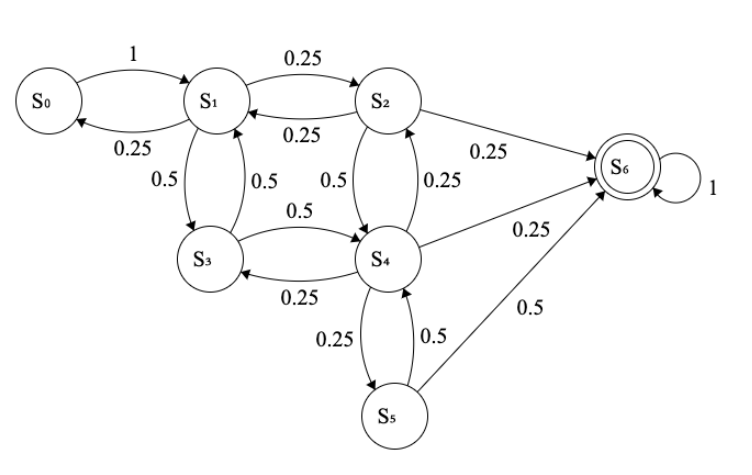
\includegraphics[width=0.5\linewidth]{fsm.png}
\end{figure}  

And the corresponding transition matrix is 

\begin{equation}
    P = \begin{bmatrix}
         0& 1 & 0 & 0 & 0 & 0 & 0 \\
         \frac{1}{4} & 0 & \frac{1}{4}  & \frac{1}{2} & 0 & 0 & 0 \\
         0 & \frac{1}{4} & 0 &0 & \frac{1}{2} & 0 & \frac{1}{4} \\
         0 & \frac{1}{2} & 0 & 0 & \frac{1}{2} & 0 & 0 \\
         0 & 0 & \frac{1}{4} & \frac{1}{4} & 0 & \frac{1}{4} & \frac{1}{4} \\
         0 & 0&0&0  &\frac{1}{2} & 0 & \frac{1}{2} \\
         0&0&0&0&0&0&1 
    \end{bmatrix} = \begin{bmatrix}
        \boldsymbol{Q} &  \boldsymbol{R} \\
        \boldsymbol{0} & 1
    \end{bmatrix}
\end{equation}

So the expectation of absorbing time is,

\begin{equation}
    (\boldsymbol{I}-\boldsymbol{Q})^{-1}\cdot \boldsymbol{1} = (\frac{135}{13},\frac{122}{13},\frac{80}{13},\frac{17}{2},\frac{73}{13},\frac{99}{26})
\end{equation}

$\E[T] = \frac{135}{13}$.

To find $\bP(X_T = 3,Y_T=0)$, first notice that $\bP(X_T=3,Y_T=0) = \bP(X_T=0,Y_T=3) = \bP(X_T=-3,Y_T=0) =\bP(X_T=0,Y_T=-3) = \frac{1}{4} \bP(M_T=3,m_T=0)$. Then we can divide $S_6= \{M_n= 3\}$ into $3$ states which are also absorbing,

\begin{itemize}
    \item $S_6^{(0)}= \{M_n= 3,m_n=0\}$
    \item $S_6^{(1)}= \{M_n= 3,m_n=1\}$
    \item $S_6^{(2)}= \{M_n= 3,m_n=2\}$
\end{itemize}

Thus the corresponding matrix $\boldsymbol{R}$ is,

\begin{equation}
    \begin{bmatrix}
        0&0&0\\
        0&0&0\\
        \frac{1}{4} & 0 &0 \\
        0&0&0\\
        0&\frac{1}{4}&0 \\
        0 & 0 & \frac{1}{2}
    \end{bmatrix}
\end{equation}

The absorbing probability is, 

\begin{equation}
    (\boldsymbol{I}-\boldsymbol{Q})^{-1}\cdot \boldsymbol{R} = \begin{bmatrix}
        \frac{4}{13}&\frac{6}{13}&\frac{3}{13}\\
        \frac{4}{13}&\frac{6}{13}&\frac{3}{13}\\
        \frac{11}{26}&\frac{5}{13}&\frac{5}{26} \\
        \frac{1}{4}&\frac{1}{2}&\frac{1}{4}\\
        \frac{5}{26}&\frac{7}{13}&\frac{7}{26}\\
        \frac{5}{52}&\frac{7}{26}&\frac{33}{52}
    \end{bmatrix}
\end{equation}

So $\bP(X_T=3,Y_T=0) = \frac{1}{4} \times \frac{4}{13} = \frac{1}{13}$


\subsection{(ii)}

Using the same method in (i), define the states as follow, 

\begin{itemize}
    \item $S_0 = \{|X_n|+|Y_n| = 0\}$
    \item $S_1 = \{|X_n|+|Y_n| = 1\}$
    \item $S_2 = \{|X_n|+|Y_n| = 2, \big| |X_n|-|Y_n|\big|=2\}$
    \item $S_3= \{|X_n|+|Y_n| = 2, \big| |X_n|-|Y_n|\big|=0\}$
    \item $S_4 = \{|X_n|+|Y_n| = 3\}$
\end{itemize}

And we have an absorbing markov chain as follow.
\begin{figure}[!htbp]
    \centering
    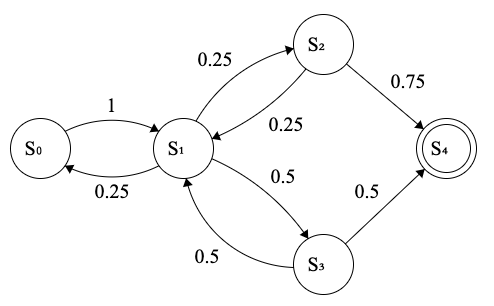
\includegraphics[width=0.5\linewidth]{fsm-2.png}
\end{figure}  

We define the expectation of steps from $S_i$ to reach $S_3$ as $f_i,i=0,1,2$.

\begin{equation}
    \left\{
        \begin{aligned}
            &f_0 = f_1 +1 \\
            &f_1 = 0.25f_0+0.25 f_2+0.5f_3+ 1 \\ 
            &f_2 = 0.25 f_1 + 1 \\
            & f_3 = 0.5f_1+1
        \end{aligned}
    \right.
\end{equation}

Solving the equation we have $\E[T] = f_0 = \frac{39}{7}$. (It is equivalent to $(\boldsymbol{I}-\boldsymbol{Q})^{-1}\cdot \boldsymbol{1}$.)

Also we can split $S_4$ into two sub states,
\begin{itemize}
    \item $S_4^{(0)} = \{|X_n|+|Y_n| = 3, \big| |X_n|-|Y_n|\big|=3\}$
    \item $S_4^{(1)} = \{|X_n|+|Y_n| = 3, \big| |X_n|-|Y_n|\big|=1 \}$
\end{itemize}

And the corresponding matrix $\boldsymbol{R}$ is

\begin{equation}
    \begin{bmatrix}
        0 & 0 \\
        0 & 0\\
        0.25 & 0.5 \\
        0 & 0.5 \\
    \end{bmatrix}
\end{equation}

The absorbing probability is, 

\begin{equation}
    (\boldsymbol{I}-\boldsymbol{Q})^{-1}\cdot \boldsymbol{R} = \begin{bmatrix}
        \frac{1}{7} & \frac{6}{7} \\
        \frac{1}{7} & \frac{6}{7} \\
        \frac{2}{7} & \frac{5}{7} \\
        \frac{1}{14} & \frac{13}{14} 
    \end{bmatrix}
\end{equation}

So $P(X_T=3,Y_T=0) = \frac{1}{4} P(|X_T|+|Y_T| = 3, \big| |X_T|-|Y_T|\big|=3) = \frac{1}{28}$.


\subsection{(iii)}
% First we limit the area of random walk within $-2\leqslant X \leqslant 2N+2, -2\leqslant Y \leqslant 2 $.
Define the expectation steps from $(X_n = x,Y_n= y)$ to first arrive at the boundary as $f(x,y)$.

\begin{equation}
    \left\{
        \begin{aligned}
            &f(-2,y) = f(x,2) = f(x,-2) = 0\\
            &f(x,y) = \frac{1}{4}[f(x-1,y)+f(x+1,y)+f(x,y-1)+f(x,y+1)] +1 
        \end{aligned}
    \right.
\end{equation}

According to symmetry we have $f(x,-1) = f(x,1)$.


Define $g_i=f(i,0),h_i = f(i,-1)= f(i,1)$. We have

\begin{equation}
    \left\{
        \begin{aligned}
            &g_{-2} = h_{-2} = 0 \\
            & g_{i} = 0.5 h_{i} + 0.25 g_{i-1} + 0.25 g_{i+1} + 1 \\
            & h_{i} =  0.25 h_{i-1}+0.25 h_{i+1} + 0.25 g_{i} + 1 % & g_{n} = 0.5 h_{n} + 0.p5 g_{n-1} +1 \\ % & h_{n} = 0.25 g_{n} + 0.5 h_{n-1}+1
        \end{aligned}
    \right.
\end{equation}

Because $\lim\limits_{n\to \infty} g_{n+1}-g_{n} = 0$, we have $\lim\limits_{n\to \infty} g_{n} = 8, \lim\limits_{n\to \infty} h_n = 6$. Denote $\alpha_i = g_i - 8,\beta_i = h_i - 6$. 

\begin{equation}
    \alpha_i + \sqrt{2}\beta_i = \frac{4+\sqrt{2}}{14} (\alpha_{i-1} + \sqrt{2}\beta_{i-1}) + \frac{4+\sqrt{2}}{14} (\alpha_{i+1} + \sqrt{2}\beta_{i+1})
\end{equation}

\begin{equation}
    \alpha_i -\sqrt{2}\beta_i = \frac{4-\sqrt{2}}{14} (\alpha_{i-1} - \sqrt{2}\beta_{i-1}) + \frac{4-\sqrt{2}}{14} (\alpha_{i+1} -\sqrt{2}\beta_{i+1})
\end{equation}

We have 

\begin{equation}
    \begin{aligned}
        \alpha_n + \sqrt{2} \beta_i = A_1 \lambda_1 ^n + A_2 \lambda_2^n  \\
        \alpha_n - \sqrt{2} \beta_i = B_1 \mu_1 ^n + A_2 \mu_2^n 
    \end{aligned}
\end{equation}

where $\lambda_{1,2} = \frac{1}{2} (4-\sqrt{2}\pm \sqrt{14-8\sqrt{2}} ),\mu_{1,2} = \frac{1}{2} (4+\sqrt{2}\pm \sqrt{14+8\sqrt{2}} )$. Because $\lim\_{n\to \infty} \alpha_n = \lim_{n\to \infty}\beta_n = 0 $, we have $A_1 = B_1 = 0$, thus 

\begin{equation}
    \begin{aligned}
        \alpha_{n}  = \frac{1}{2} \left( A \lambda^n + B \mu^n \right) \\
        \beta_{n}  = \frac{1}{2\sqrt{2}} \left( A \lambda^n - B \mu^n \right)
    \end{aligned}
\end{equation}

where $\lambda = \frac{1}{2} (4-\sqrt{2}- \sqrt{14-8\sqrt{2}} ),\mu = \frac{1}{2} (4+\sqrt{2}-\sqrt{14+8\sqrt{2}} ).$

And $\alpha_{-2} = g_{-2} - 8 = -8,\beta_{-2} = h_{-2}-6 =  - 6 $, we have $A = -\lambda^2 (8+6\sqrt{2}),B =\mu^2(6\sqrt{2}-8)$.

\begin{equation}
    g_0 = \alpha_0 + 8 = \frac{1}{2}(A+B) + 8 = 3\sqrt{2} (\mu^2 - \lambda^2) - 4(\mu^2 + \lambda^2) + 8 =10 \sqrt{7+\sqrt{17}}-8 \sqrt{14-2 \sqrt{17}}-8 = 6.1617
\end{equation}

To solve $P(X_T=0,Y_T=0)$, similarly we need to find $ (\boldsymbol{I}-\boldsymbol{Q})^{-1}\cdot \boldsymbol{R}$. However, since the Markov chain is infinite, we can define $p(x,y)$ as $P(X_T=0,Y_T=0|X_0=x,Y_0 = y)$ and solve the following equation,

\begin{equation}
    \left\{
        \begin{aligned}
            &p(-2,0) = 1 \\
            &p(-2,-1) = p(-2,1) = p(x,2) = p(x,-2) = 0 \\
            &p(x,y) = \frac{1}{4}[p(x-1,y)+p(x+1,y)+p(x,y-1)+p(x,y+1)]
        \end{aligned}
    \right.
\end{equation}

Follows the same step, we have $P(X_T = -2,Y_T=0) = p(0,0) = \frac{1}{2} (\lambda^2 + \mu^2) = 16 - \sqrt{2 (95+7\sqrt{17})} = 0.1304$.


\subsection{(iv)}

\section{Problem 7}

\subsection{(i)}

First, for a random variable $X,\E[X]=0$ and there exists some constant $\alpha$, such that $\E[e^{tx}] \leqslant e^{\alpha^2 t^2/2}$, then $X$ is sub-Gaussian, and we have that 

\begin{equation}
    \bP(X \geqslant \lambda )  =  P(e^{tX} \geqslant e^{t\lambda} ) \leqslant \frac{E[e^{tX}]}{e^{t\lambda}} \leqslant e^{\alpha^2t^2/2 - t\lambda}
\end{equation}

Let $t= \frac{\lambda}{\alpha}$, we have

\begin{equation}
    \bP(X \geqslant \lambda ) \leqslant e^{-\frac{\lambda^2}{2\alpha^2}}
\end{equation}

\begin{equation}
    \bP(|X| \geqslant \lambda ) \leqslant 2e^{-\frac{\lambda^2}{2\alpha^2}}
\end{equation}

For $X_i$, we have $\E[\exp(tX_i)]  =\frac{1}{2} (e^t + e^{-t})\leqslant \exp(t^2/2)$.
When $\sum\limits_{i=1}^{\infty} a_i^2 = S < \infty$,

\begin{equation}
    \E[\exp(\sum_{i=1}^{\infty} a_iX_it) ] = \prod_{i=1}^{\infty} \E[\exp(ta_iX_i)] \leqslant  \prod_{i=1}^{\infty} \exp(t^2a_i^2)= e^{St^2}
\end{equation}

Denote $X= \sum_{i=1}^{\infty} a_iX_i$, 


\begin{equation}
    \bP(|X| \geqslant \lambda)  \leqslant 2e^{-\frac{\lambda^2}{S}}
\end{equation}

Thus we have $X$ converges almost surely, i.e $\bP(|X| \leqslant \infty) = \bP(|\sum_{i=1}^{\infty} a_iX_i| < \infty) = 1$.

\subsection{(ii)}

By the corollary of Kolmogorov three-series theorem, given independent variables $X_1,X_2,\cdots,X_n$,

\begin{equation}
    \bP\left(\sum_{k=1}^{\infty} X_{k} \text { converges }\right)=0 \text { or } 1
\end{equation}

And because $\E[(\sum_{i=1}^{\infty} a_iX_i)^2] = \sum_{i=1}^{\infty} a_i^2 = \infty$, $\bP(|\sum_{i=1}^{\infty} a_iX_i| = \infty) >0$, thus 

\begin{equation}
    \bP\left(\big|\sum_{i=1}^{\infty} a_iX_i \big| < \infty\right) = 0
\end{equation}


\section{Problem 8}

\subsection{(i)}

It is easy to see that $Y_n = (X_{n-1},X_n)$ is a Markov Chain. And $Y_1 = (0,1)$. Thus $Y_2 = (1,1)$. And the state transition graph is as follow.

\begin{figure}[!htbp]
    \centering
    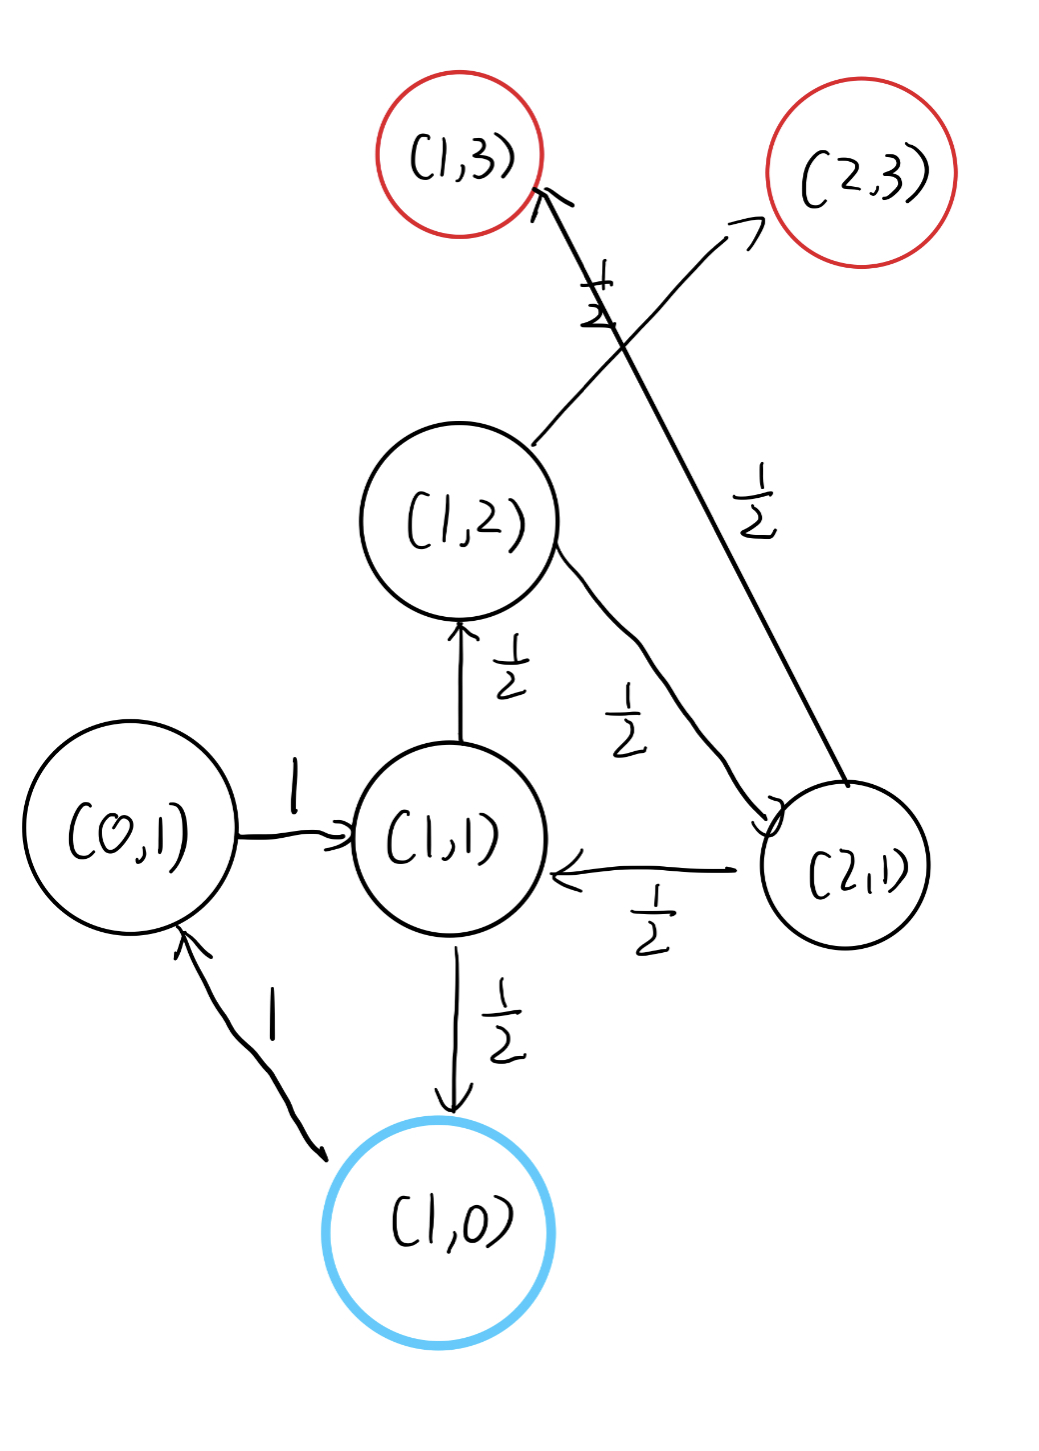
\includegraphics[width=0.4\linewidth]{State.jpg}
\end{figure}

So if $X_n$ reaches 0 before 3, the path is consisted of three parts,

\begin{itemize}
    \item $(0,1)\to (1,1)$
    \item $m$ (can be zero) circles of $(1,1) \to (2,1) \to (1,2) \to (1,1)$ 
    \item $(1,1)\to (1,0)$
\end{itemize}

So 

\begin{equation}
    \bP(X_n \text{ reaches } 0 \text{ before } 3) = \sum_{m=0}^{\infty} \frac{1}{2} (\frac{1}{8})^m = \frac{4}{7}
\end{equation}

Thus

\begin{equation}
    \bP(X_n \text{ reaches } 3 \text{ before } 0) = 1-\frac{4}{7} = \frac{3}{7}
\end{equation}

\subsection{(ii)}

$Y_1 = (1,2)$. Denote $p$ as the hitting probability of $(1,1)$ from $(1,2)$ and $q$ as the hitting probability of $(1,1)$ from $(2,1)$. Consider the Markov chain starting from $(1,2)$ and $(2,1)$, it can be expressed as a binary tree with recursive structure.

\begin{figure}[!htbp]
    \centering
    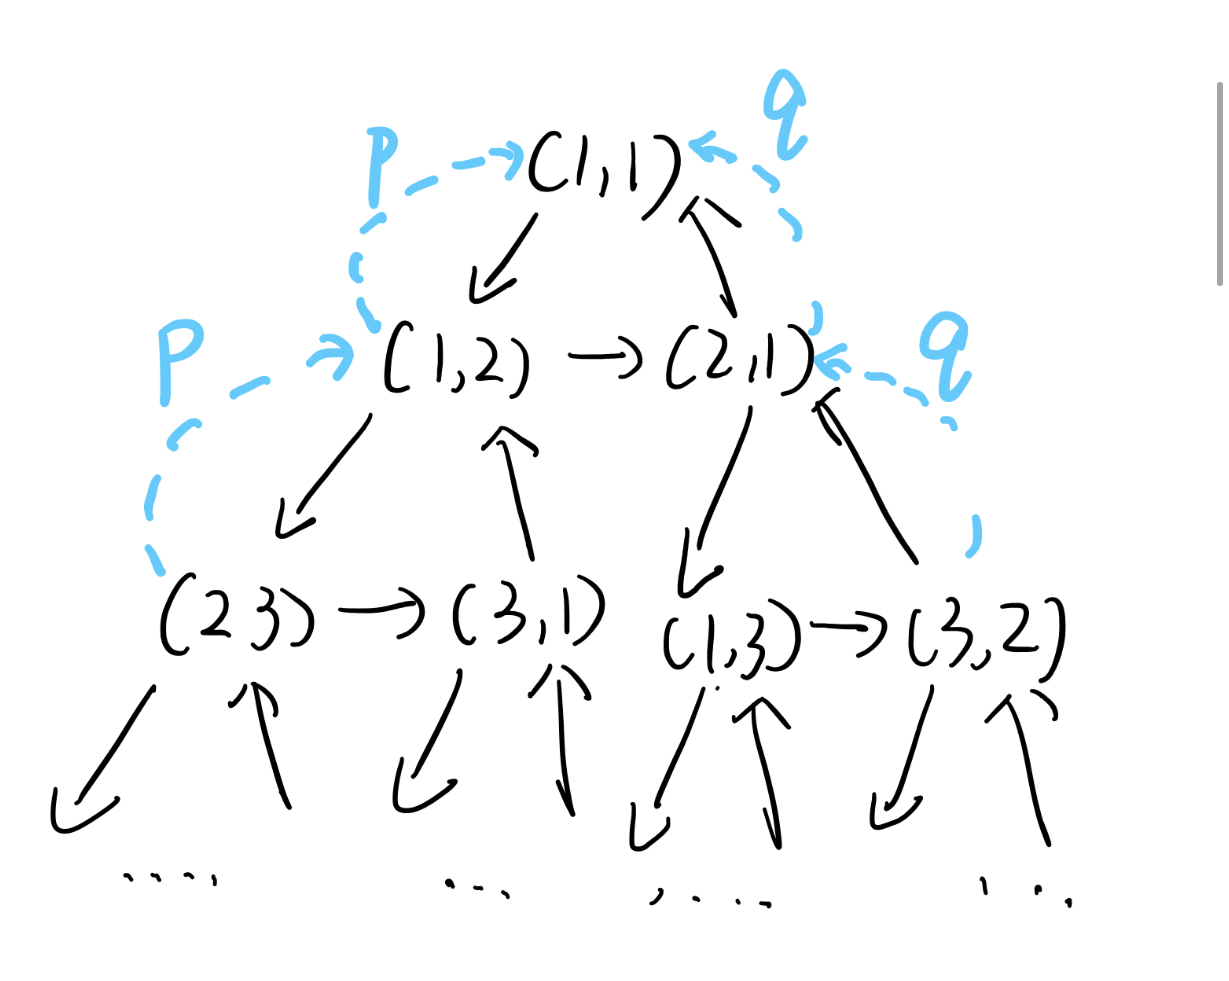
\includegraphics[width=0.4\linewidth]{s.jpg}
\end{figure}

So we have

\begin{equation}
    \left\{
        \begin{aligned}
            &p = \frac{1}{2} q + \frac{1}{2} p^2 \\
            &q = \frac{1}{2} + \frac{1}{2} pq
        \end{aligned}
    \right.
\end{equation}

We have $p(2-p)^2 = 1$. Because $p\leqslant 1$ we have $p = 1$ or $\frac{3-\sqrt{5}}{2}$. 

Notice that 

\begin{equation}
    \bP\left(\exists n ,Y_n = (1,1) | Y_0 = (1,2)\right) = \bP\left(Y_n = (1,1) | Y_{n-1} = (2,1)\right)\bP\left(\exists n ,Y_{n-1} = (2,1) | Y_0 = (1,2)\right) \leqslant \frac{1}{2}
\end{equation}

So $p = \frac{3-\sqrt{5}}{2}$.


% Denote $S_k = \s
% Denote $S_k = \sum_{i=0}^k Y_i$ and $S_0 = 0$

% \begin{equation}
%     f(n) = \sum_{k=0}^{\infty} P(S_k = n) 
% \end{equation}

% Notice that $P(S_n = k) = 0$ for $n>k$,

% \begin{equation}
%     \begin{aligned}
%         f(n) & = \sum_{k=0}^{n} åP(S_k = n) = \sum_{k=1}^{n} \sum_{j=0}^{n-1} P(S_{k-1} = j,Y_k = n-j) \\
%         & = \sum_{j=0}^{n-1} p_{n-j}\sum_{k=1}^{n}  P(S_{k-1} = j) = \sum_{j=0}^{n-1} p_{n-j} f(j)
%     \end{aligned}
% \end{equation}

% Denote $f_n= f(n)$ and $f_0 = 0$ and the genetating function of $f_n$ and $p_n$ is

% \begin{equation}
%     F(z) = \sum_{i=0}^{\infty} f_i z^i, \quad P(z) = \sum_{i=1}^{\infty} p_i z^i
% \end{equation}

% We have

% \begin{equation}
%     F(z)-1 = \sum_{n=1}^{\infty} f_n z^n = \sum_{n=1}^{\infty} \sum_{j=0}^{n-1} p_{n-j} f_j z^{n} = (\sum_{j=0}^{\infty} f_{j}z^j ) (\sum_{i=1}^{\infty} p_i z^i) = F(z) U(z)
% \end{equation}

% So 

% \begin{equation}
%     F(z) = \frac{1}{1-U(z)}
% \end{equation}


\end{document} 
